\documentclass[a4paper,12pt]{article} 
\usepackage{geometry}
\usepackage{wrapfig}
\geometry{
	a4paper,
	total={170mm,257mm},
	left=10mm,
	right=10mm,
	top=20mm,
}
\usepackage{titlesec}
\titlelabel{\thetitle.\quad} %точка в section

%%% Работа с русским языком
\usepackage{cmap}                           % поиск в PDF
\usepackage{mathtext} 			 	       % русские буквы в формулах
\usepackage[T2A]{fontenc}               % кодировка
\usepackage[utf8]{inputenc}              % кодировка исходного текста
\usepackage[english,russian]{babel}  % локализация и переносы

%Математика
\usepackage{amsmath,amsfonts,amssymb,amsthm,mathtools} % AMS
\usepackage{icomma} % "Умная" запятая

%% Шрифты
\usepackage{euscript}	 % Шрифт Евклид
\usepackage{mathrsfs} % Красивый матшрифт

\usepackage{gensymb}
\usepackage{graphicx}
\usepackage{setspace}
\usepackage{tabularx}
\usepackage{longtable}
\usepackage{icomma}
\usepackage{euscript}
\usepackage{float}
\usepackage{cutwin}
\usepackage{adjustbox}
\usepackage{dashbox}
\usepackage[normalem]{ulem}	
\usepackage[babel=true]{microtype}
\RequirePackage[T1]{fontenc}
\usepackage{amsmath,amsfonts,amssymb,amsthm,mathrsfs,mathtools} 
\usepackage{xcolor}         
\usepackage{enumitem}     
\usepackage{xpatch}       
\usepackage{cancel}                  
\usepackage{upgreek}                 
\usepackage{lipsum}                  
\usepackage[version=4]{mhchem}       
\usepackage{multirow}                
\usepackage{stackengine}             
\usepackage{tikz}         
\usepackage{hyperref}
\hypersetup{colorlinks=true,urlcolor=blue}       
\usetikzlibrary{positioning}         
\usepackage{titletoc}                 
\usepackage{chngcntr}              
\usepackage{fancyhdr}                
\usepackage{makecell}                
\usepackage{indentfirst}             
\usepackage{tocloft}                 
\usepackage{soul}                   
\usepackage[stable]{footmisc}       
\usepackage{subfig}  
\usepackage{comment}                  


\mathtoolsset{showonlyrefs=true}


\theoremstyle{definition}
\newtheorem*{definition}{Определение}
\newtheorem{statement}{Предложение}[section]
\newtheorem{lemma}{Лемма}[section]
\newtheorem{theorem}{Теорема}[section]
\newtheorem*{theoremn}{Теорема}
\newtheorem*{corollary}{Следствие}
\newtheorem*{example}{Пример}
\newtheorem*{note}{Замечание}
\newtheorem*{problem}{Задача}


\counterwithout{footnote}{section}\DeclareRobustCommand{\divby}{%
	\mathrel{\text{\vbox{\baselineskip.65ex\lineskiplimit0pt\hbox{.}\hbox{.}\hbox{.}}}}%
}

\newcommand{\dotpr}[2]{\bra{#1}\ket{#2}}
\let\AA\relax
\let\emptyset\varnothing
\DeclareMathOperator*{\esssup}{ess sup}
\DeclareMathOperator*{\ord}{ord}
\DeclareMathOperator*{\supp}{supp}
\DeclareMathOperator*{\pr}{pr}
\DeclareMathOperator*{\Ker}{Ker}
\DeclareMathOperator*{\Vol}{Vol}
\DeclareMathOperator*{\rg}{rk}
\DeclareMathOperator*{\Ima}{Im}
\DeclareMathOperator*{\Alt}{Alt}
\DeclareMathOperator*{\Sym}{Sym}
\newcommand{\eqdef}{\stackrel{\text{\tiny{def}}}{=}}
\newcommand{\pp}{\partial}
\newcommand{\AA}{\mathcal{A}}
\newcommand{\BB}{\mathcal{B}}
\newcommand{\MM}{\mathbb{M}}
\newcommand{\NN}{\mathbb{N}}
\newcommand{\ZZ}{\mathbb{Z}}
\newcommand{\QQ}{\mathbb{Q}}
\newcommand{\RR}{\mathbb{R}}
\newcommand{\CC}{\mathbb{C}}
\newcommand{\FFF}{\mathbb{F}}
\newcommand{\DD}{\mathcal{D}}
\newcommand{\FF}{\mathcal{F}}
\newcommand{\sS}{\mathcal{S}}
\newcommand*\circled[1]{\tikz[baseline=(char.base)]{
		\node[shape=circle,draw,inner sep=2pt] (char) {#1};}}

%%% Заголовок
\author{Шерхалов Денис Б02-204и}
\title{Лабораторная работа 4.2.3 \\
	\textbf{Исследование показателей преломления \\
    с помощью интерферометра Релея}}
\date{9 апреля 2024 г.}

\begin{document}
	
{\Large \maketitle}

	\paragraph*{Цель работы:} Знакомство с техникой интерференционных измерений показателей преломления газов с помощью интерферометра Релея.
	\paragraph*{В работе используются:} интерферометр Релея, газовая кювета, осветитель, зрительная труда, сильфон, баллон с углекислым газом, манометр, краны, светофильтр

\section{Введение}

В одну из камер вводится исследуемый газ, а вторая заполнена воздухом при атмосферном давлении. При этом разность хода $\Delta$, вызванная разностью показателей преломления газов $\delta n$, приводит к сдвигу интерференционных полос:
\begin{equation}
    \Delta = \delta n \cdot l \quad \Rightarrow \quad \delta n = m \frac{\lambda}{l},
\end{equation}
так как сдвиг на одну полосу соответствует дополнительной разности хода $\Delta = \lambda$.
\par Показатель преломления исследуемого газа определяется путем сравнения с воздухом при атмосферном давлении:
\begin{equation}
    n = n_{air} + \dfrac{\Delta}{l}
\end{equation}

\subsection*{Зависимость показателя преломления газа от давления и температуры} 
Молекулярная оптика устанавливает следующее простое соотношение между показалелем преломления газа и его плотностью:

$$n = \sqrt{\varepsilon} = \sqrt{1 + 4 \pi N \alpha} \approx 1+2 \pi N \alpha$$

где $N$ -- число молекул в единице объёма, $\alpha$ -- поляризуемость молекулы $(\textbf{p} = \alpha \textbf{E})$,
$\textbf{p}$ -- дипольный момент молекулы. Принимая во внимание соотношение $P = N k_B T$, получим
$$n - 1 = 2 \pi \alpha \dfrac{P}{k_B T} \quad \Rightarrow \quad \delta n = \dfrac{2 \pi \alpha}{k_B T} \Delta P$$

\par Величина $\delta n$ измеряется с помощью интерферометра Жамена, $\Delta P$ --
c помощью манометра. Одновременное измерение этих величин (и температуры $Т$)
позволяет определить поляризуемость молекул воздуха и, следовательно, рассчитать 
по формуле показатель преломления воздуха для любых значений $P$ и $T$.
Следует отметить, что воздух является смесью нескольких газов, поэтому под 
поляризуемостью молекул воздуха, нужно понимать некоторую среднюю величину,
определяемую соотношением

$$\alpha = \dfrac{1}{N} \sum_{i} \alpha_{i} N_i$$

где $\alpha_{i}$ и $N_i$ -- поляризуемость и концентрация молекул различных газов, 
входящих в состав воздуха, $N$ -- общее число молекул в единице объёма.

\par Формула позволяет установить связь показателя преломления газа $n$ при
температуре $Т$ и давлении $Р$ с показателем преломления $n_0$ при нормальных условиях ($T_0 = 273$ К, $P_0 = 1$ атм):

$$ \dfrac{n_0 - 1}{n - 1} = \dfrac{T}{T_0} \dfrac{P_0}{P} $$

\subsection*{Экспериментальная установка}
\par Интерферометр Релея — прибор
для измерения разности показателей преломления — основан на яв-
лении дифракции света на двух параллельных щелях. Схема прибора
представлена на рис. 1 в вертикальной и горизонтальной проекциях.
Лампа накаливания Л с помощью конденсора K ярко освещает узкую
входную щель $S$, расположенную в фокусе объектива $O_1$ (фокусное
расстояние $f$). Коллиматор, состоящий из щели $S$ и объектива $O_1$ , по-
сылает параллельный пучок на диафрагму $D$ с двумя вертикальными
щелями (расстояние между щелями $d$). Свет после двойной щели про-
ходит кювету L, состоящую из двух одинаковых стеклянных камер, в
которые вводятся исследуемые газы (в нашей установке — $CO_2$ или
воздух). Кювета занимает только верхнюю часть пространства между
объективами $O_1$ и $O_2$ , длина кюветы $l$. За кюветой расположены две
стеклянные пластинки $J$ (компенсатор Жамена, см. ниже) и пластин-
ка П.
Интерференционная картина (картина дифракции на двух щелях),
наблюдаемая в фокальной плоскости $F$ объектива $O_2$ , представляет со-
бой две системы равноотстоящих полос, параллельных щелям: верхняя

\par На пути луча расположен компенсатор Жамена, состоящий из двух
одинаковых плоскопараллельных стеклянных пластинок. Если обе
пластинки установлены под одинаковым углом к лучам, то и оптическая длина
пути в них для обоих лучей оказывается одинаковой. Поворот одной из пластинок
вокруг горизонтальной оси вызывает увеличение или уменьшение оптической длины
пути соответствующего луча. Это позволяет скомпенсировать разность хода,
возникающую в камерах. Для точного отсчёта угла поворота одна из пластинок
снабжена рычагом, конец которого смещается при помощи микрометрического
винта $B$. Плас тинки компенсатора ставятся под углом $45^{\circ}$ к горизонтали, что иоз-
воляет использовать линейную экстраполяцию при измерениях. Смещение полос
можно наблюдать через зрительную трубу $T$.

\begin{figure}[H]
    \centering
    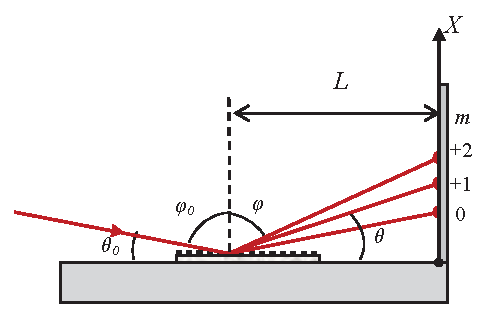
\includegraphics[width=19cm]{pic1.png}
\end{figure}

\section{Ход работы}

\begin{enumerate}
    \item Ознакомимся с принципом работы установки. Проведём юстировку и калибровку прибора. Для калибровки наденем на окуляр красный светофильтр и снимем зависимость показаний микрометрической шкалы компенсатора Жамена от порядкового номера интерференционного максимума. Результаты измерений занесём в таблицу 1 и графически представим на рис. 2
 
    
    \begin{table}[h]
        \centering
        \caption{Калибровка компенсатора.}
        \begin{tabular}{|*{12}{l|}} \hline
            $N$ полосы & $0$ & $1$ & $2$ & $3$ & $4$ & $5$ & $6$ & $7$ & $8$ & $9$ & $10$ \\ \hline
            $z_m$ & 324 & 356 & 388 & 420 & 452 & 484 & 516 & 548 & 580 & 612 & 644 \\ \hline
        \end{tabular}
    \end{table}
    
\begin{figure}[h]
    \centering
    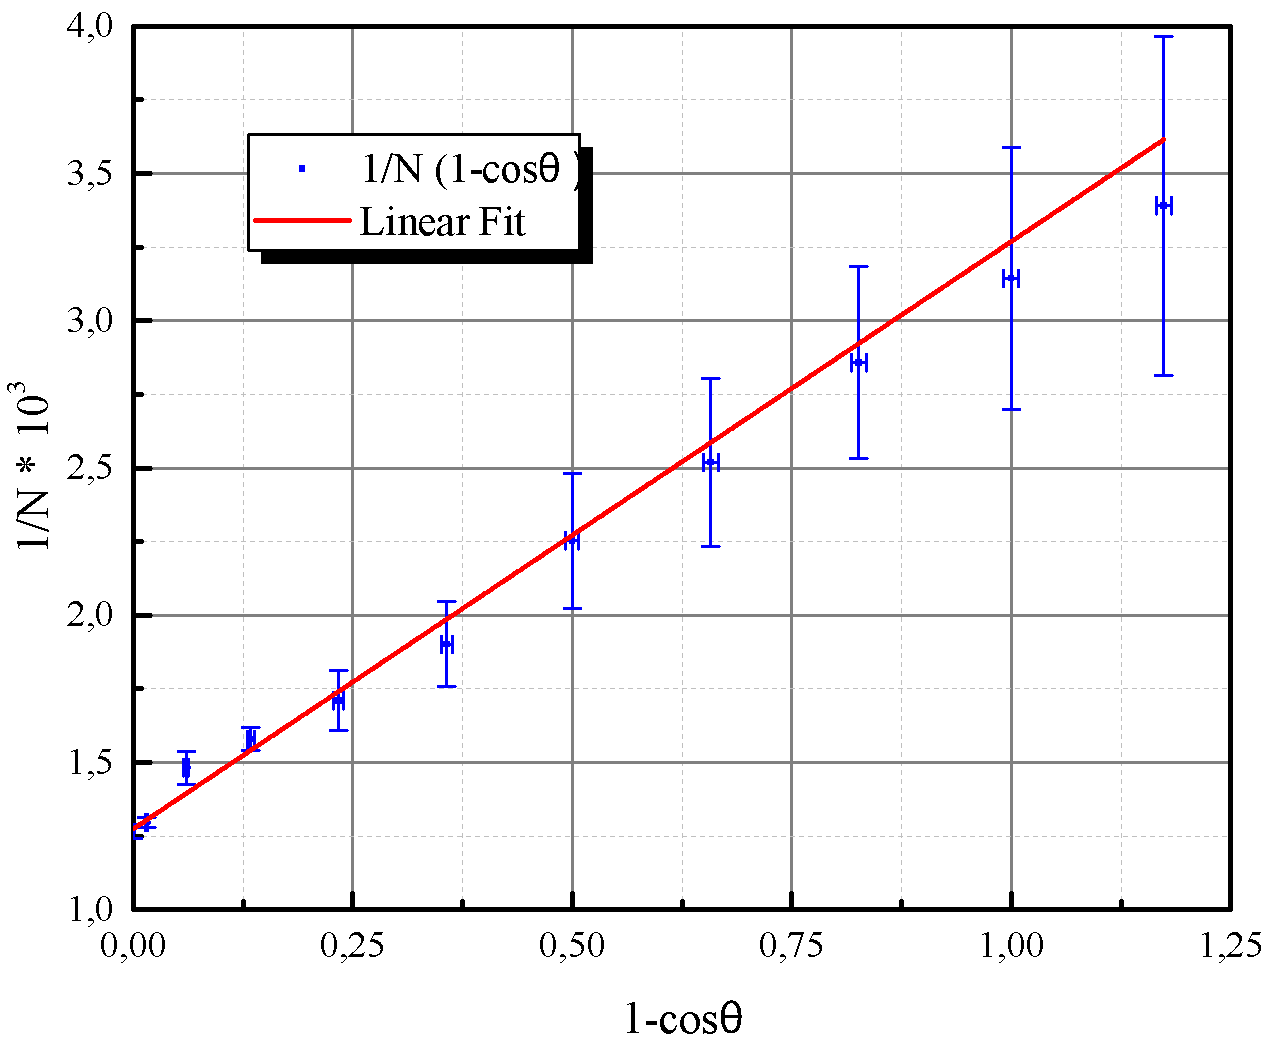
\includegraphics[width=19cm]{graph1.png}
    \caption{График калибровки компенсатора}
    \label{fig:vac}
\end{figure}

При этом длина кюветы $l_{кювета} = 10$ см, а длина волны, пропускаемая светофильтром $\lambda = 620 \div 720$ нм -- в среднем $\lambda \approx 670$ нм. Тогда $32$ деления компенсатора соответствуют $670$ нм. 

\item По формуле перейдём от делений компенсатора к величине $\delta n$:
\begin{equation}
    \delta n = m\frac{\lambda}{l},
\end{equation}
при этом из графика 1: $\Delta m = \frac{\Delta z}{\tg \varphi_1}$, где $\tg \varphi_1 = 32$ -- угол наклона калибровочного графика. Тогда окончательно

\begin{equation}
    \delta n = \frac{\Delta z}{\tg \varphi_1} \frac{\lambda}{l} = 2.1 \cdot 10^{-7} \, \Delta z
\end{equation}

\item Изменяя давление с помощью сильфона, снимем зависимость показаний компенсатора $z$ от перепада давлений $\Delta P$. Результаты занесём в таблицу 2.

\begin{table}[h]
    \centering
    \caption{Зависимость показаний микрометра от давления}
    \begin{tabular}{|*{9}{l|}} \hline
        $P$, кПа & $0$ & $-1$ & $-2$ & $-3$ & $-4$ & $-5$ & $-6$ & $-7$ \\ \hline
        $z$ & 319 & 332 & 346 & 360 & 369 & 388 & 400 & 412 \\ \hline   
    \end{tabular}
    \begin{tabular}{|*{10}{l|}} \hline
        $P$, кПа & $1$ & $2$ & $3$ & $4$ & $5$ & $6$ & $7$ & $8$ \\ \hline
        $z$ & 304 & 296 & 273 & 259 & 246 & 231 & 218 & 203 \\ \hline   
    \end{tabular}
\end{table}

\begin{figure}[h]
    \centering
    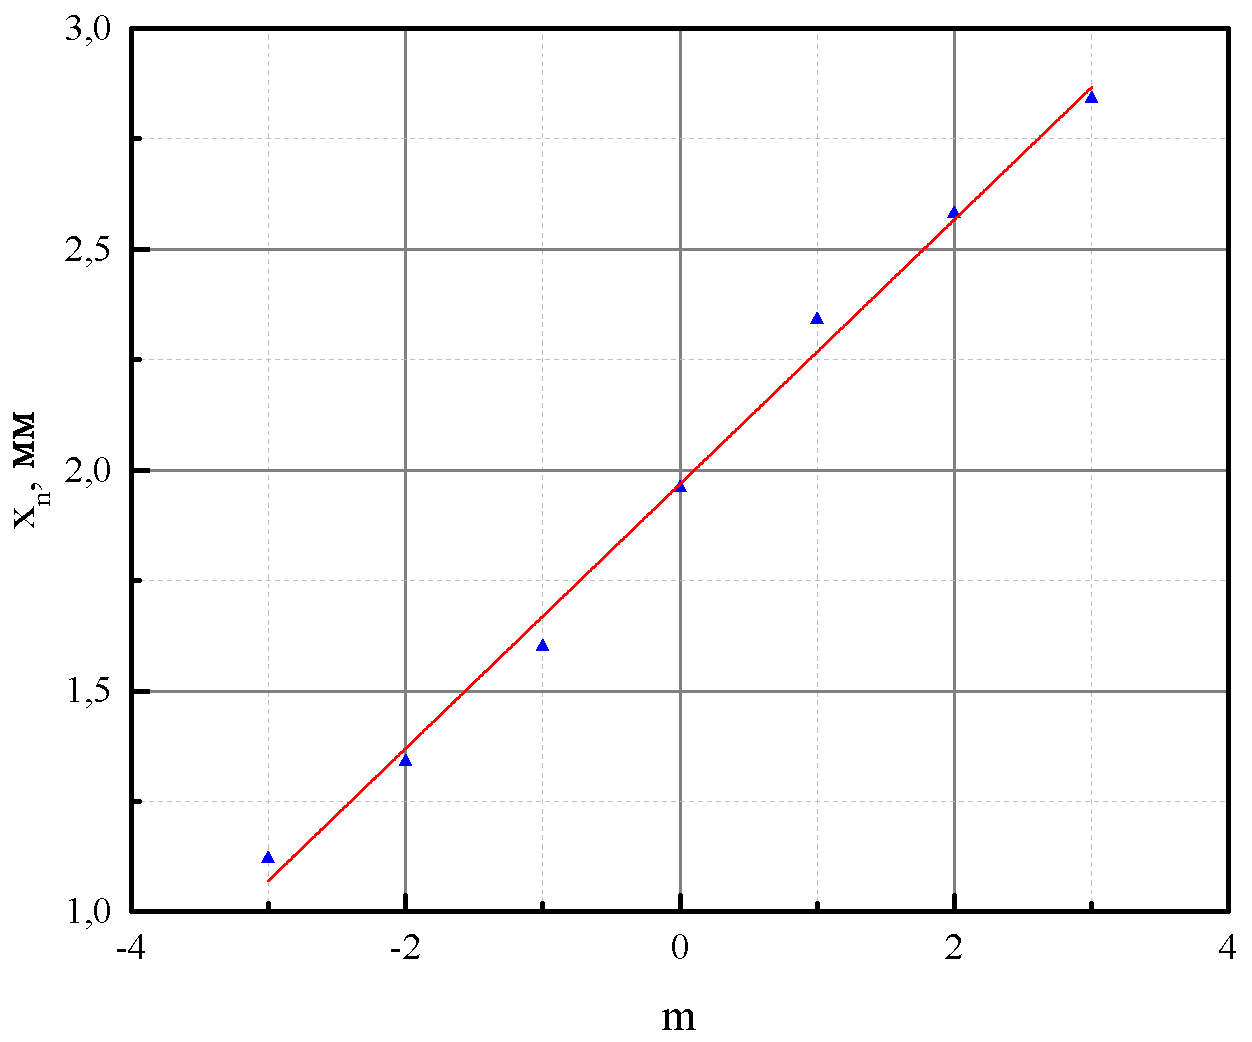
\includegraphics[width=19cm]{graph2.png}
    \caption{Зависимость показаний микрометра от давления}
\end{figure}

Угол наклона графика $\tg \varphi_2 = 14.0 \, \dfrac{\text{дел}}{\text{кПа}}$

\item Определим среднюю поляризуемость молекулы воздуха:

\begin{equation}
\delta n = \frac{2 \pi \alpha}{k_B T} \Delta P
\end{equation}

\begin{equation}
\alpha = \frac{\delta n k_B T}{2 \pi \Delta P} = \frac{\Delta z \lambda}{\tg \varphi_1 l} \frac{k_B T}{2 \pi \Delta P} =\frac{\tg \varphi_2}{\tg \varphi_1} \frac{\lambda k_B T}{2 \pi l} = 176 \cdot 10^{-32}
\end{equation}

Табличное значение составляет $\alpha = 172 \cdot 10^{-32}$

Погрешность измерения определим по стандартной формуле (умножение величин), погрешность измерения углов наклона определим методом наименьших квадратов.
\begin{equation}
\varepsilon_{\alpha} = \sqrt{(\frac{\sigma_{\tg \varphi_2}}{\tg \varphi_2})^2 + (\frac{\sigma_{\tg \varphi_1}}{\tg \varphi_1})^2 + (\frac{\sigma_{T}}{T})^2 + (\frac{\sigma_{l}}{l})^2 + (\frac{\sigma_{\Delta P}}{\Delta P})^2} = 3.1\%
\end{equation}

\item Определим показатель преломления воздуха по формуле
\begin{equation}
    n_0 = 1 + 2\pi\alpha \frac{P_0}{kT_0} = 1.000293
\end{equation}

Для $T = 295$ K и $P = 101.6$ кПа
\begin{equation}
    n = 1 + \frac{(n_0 - 1)T_0 P}{T P_0} = 1.000276
\end{equation}

Аналогично п. 4, погрешность определения показателя преломления составляет 
\begin{equation}
    \sigma_n = 0.000005 \hspace{1cm} \varepsilon = 4 \%
\end{equation}

В пределах погрешность теоретический и экспериментальный результаты совпадают.

\item По результатам измерений оценим радиус молекулы азота (из которых в основном состоит воздух), приняв молекулу за металлический шарик в однородном электрическом поле. Из задачи о проводниковом шаре в электрическом шаре, дипольный момент его будет равен $p = 3V E_0$, но в то же время $p = \alpha E$ из определения
Получили, что 
\begin{equation}
    \alpha = 3 V \quad \Rightarrow \quad r \sim \alpha^{1/3} \sim 10^{-10} \text{м}
\end{equation}

Реальный радиус молекулы азота также составляет порядка $10^{-10}$ м, наша оценка верна.

\item Во вторую кювету запустим углекислый газ. Сразу после этого набежит разность хода, которая компенсируется поднятием компенсатора на 190 мкм.

Так как $n_2 - n_1 = \delta n$, а $\delta n$ была определена по формуле через калибровочный график, $\delta n = \Delta z \frac{\lambda}{l \tg \varphi_1} = 0.995 \Delta z$

Поэтому 
\begin{equation}
    n_{CO2} = n + 0.995\Delta z = 1.000303 + 0.000179 = 1.000482 \pm 0.000032
\end{equation} 
Погрешности определены аналогично предыдущим пунктам, и в их пределах результаты практически совпадают: при данных Т и Р $n_{CO_{2}} = 1.000420$

\begin{table}[h]
    \centering
    \caption{Зависимость показаний компенсатора от времени}
    \begin{tabular}{|*{10}{l|}} \hline
        $t$, мин & $0$ & $1$ & $2$ & $3$ & $4$ & $5$ & $6$ & $7$ & $8$\\ \hline
        $z$ & 1016 & 862 & 786 & 721 & 692 & 667 & 628 & 594 & 566 \\ \hline   
    \end{tabular}
    \begin{tabular}{|*{9}{l|}} \hline
        $t$, мин  & $9$ & $10$ & $11$ & $12$ & $13$ & $14$ & $15$ & $16$ \\ \hline
        $z$ & 548 & 523 & 500 & 486 & 468 & 451 & 449 & 450 \\ \hline   
    \end{tabular}
\end{table}

Из зависимости показаний компенсатора от времени видно, что система подтекает, а время установления равновесия порядка 14 минут.
\end{enumerate}

\section{Вывод}

В ходе работы был изучен принцип работы интерферометра Релея, а также экспериментально определены следующие различные величины:
\begin{itemize}
    \item поляризуемость молекулы воздуха:
    $$\alpha_{exp} = (176 \pm 5) \cdot 10^{-32}  \hspace{2cm} \alpha_{th} = 172 \cdot 10^{-32}$$
    \item показатель преломления воздуха при $T = 295$ К и $P = 101.6$ кПа:
    $$n_{exp} = 1.000293 \pm 0.000011 \hspace{2cm} n_{th} = 1.000283$$
    \item оценен радиус молекулы азота:
    $$r \sim 10^{-10} m$$
    \item показатель преломления углекислого газа при $T = 295$ К и $P = 101.6$ кПа:
    $$n_{exp} = 1.000482 \pm 0.000032 \hspace{2cm} n_{th} = 1.000420$$
\end{itemize}

Хотя и существуют более точные интерферометры, интерферометр Релея хорошо подходит для определения этих параметров.

\end{document}